\section{Design Thinking}
\subsection{Empatía}

Cada semestre en el Club de Ajedrez de la Universidad del Valle de Guatemala, entran decenas de personas esperando inmiscuirse en el mundo del ajedrez; sin embargo, se encuentran con la barrera del desconocimiento de varios principios fundamentales de este deporte y finalmente, estas personas, terminan abandonando el club o simplemente siendo miembros inactivos. \newline\newline
La junta directiva del Club de Ajedrez ha intentando implementar diversas actividades para evitar que los miembros se vuelven inactivos; por lo cual, se busca generar un sistema de recomendaciones que ayude a los miembros del club a tener una visión más amplia del ajedrez y que este se vuelva más envolvente en sus vidas.

\subsection{Definición}
Los principales problemas identificados son: 
\begin{enumerate}
    \item Desconocimiento de las fases del ajedrez. 
    \item Desconocimiento de las estrategias adecuadas para cada nivel de juego. 
    \item Herramientas adecuadas para aprender a jugar ajedrez.
\end{enumerate}

El problema propuesto a resolver es un sistema de recomendaciones de cierto de tipo de posiciones. 

\subsection{Ideación}
Existen diversas fases en el ajedrez, sin embargo, el sistema de recomendaciones se centrará en la primera fase: la apertura. 

El propósito es encontrar las aperturas jugadas por los miembros de club que tengan el mismo nivel. Es decir, las 3 categorías: 
\begin{enumerate}
    \item Principiante 
    \item Intermedio 
    \item Avanzado 
\end{enumerate}
\subsection{Prototipos}
La primera fase se ha basado en elegir los parámetros más idóneos a evaluar, se han propuesto los más relevantes: 

\begin{enumerate}
    \item Plataforma favorita para jugar. 
    \item Plataforma con los mejores recursos para aprender. 
    \item Modalidad favoritas de juego. 
    \item Modalidad que le gusta observar en Youtube, Twitch, etc... 
    \item Parte favorita de una partida. 
    \item Su nivel de juego en Blitz.
    \item Su nivel de juego en Rápidas.
    \item Apertura que juega.
    \item Defensa que juega.
\end{enumerate}

De los cuales, únicamente se tomaron en cuenta los siguientes parámetros: 

\begin{enumerate}
    \item $PLATAFORMA$ - Plataforma favorita para jugar. 
    \item $APERTURA$ - Apertura que juega.
    \item $DEFENSA$ - Defensa que juega.
    \item $PARTE\_ FAVORITA$ - Parte favorita de una partida. 
    \item $NIVEL\_BLITZ$ - Su nivel de juego en Blitz.
    \item $NIVEL\_RAPIDAS$ - Su nivel de juego en Rápidas. 
\end{enumerate}
\subsection{Testing}
La encuesta se encuentra aquí: \textcolor{blue}{\href{https://forms.gle/5swmk2VsKMPd1hha6}{https://forms.gle/5swmk2VsKMPd1hha6}}.\newline\newline
La encuesta se basó en las siguientes preguntas: 
\begin{enumerate}
    \item Nivel de juego en blitz  (\textit{Considere un estimado de su rating en chess.com: (1) Principiante [0 a 1400 elo], (2) Intermedio [1400 - 1600 elo], (3) Avanzado [1600- infinito].}): 
    \begin{enumerate}
        \item Principiante 
        \item Intermedio 
        \item Avanzado
    \end{enumerate}
    \item Nivel de juego en rápidas (\textit{Considere un estimado de su rating en chess.com: (1) Principiante [0 a 1400 elo], (2) Intermedio [1400 - 1600 elo], (3) Avanzado [1600- infinito].}): 
    \begin{enumerate}
        \item Principiante 
        \item Intermedio 
        \item Avanzado
    \end{enumerate}
    \item ¿Cuál es tu parte favorita del ajedrez?
    \begin{enumerate}
        \item Apertura 
        \item Intermedio 
        \item Final
    \end{enumerate}
    \item ¿Cuál es tu plataforma favorita para jugar?
    \begin{enumerate}
        \item Lichess.org
        \item Chess.com
        \item Chess24.com
        \item Otro
    \end{enumerate}
    \item De las aperturas anteriores, ¿cuál se adecúa más a tu estilo de juego? 
    \begin{enumerate}
        \item Italiana/Española
        \item Inglesa
        \item Sistema Londres
        \item Fianchetto
    \end{enumerate}
    \item De las defensas anteriores, ¿cuál se adecúa más a tu estilo de juego? 
    \begin{enumerate}
        \item Eslava
        \item Francesa
        \item Caro-Kann
        \item Siciliana
    \end{enumerate}
\end{enumerate}
\subsubsection{Explicación}

Por el planteamiento del problema, la idea es que el usuario ingrese su nivel de juego (principiante, intermedio o avanzado). Entonces el programa le recomendará la plataforma, apertura y defensa de jugadores de su mismo nivel. Desde el punto de vista matemático, el programa únicamente buscará las relaciones y nodos conectados a los niveles de juego. \newline

Las aperturas y defensas en las siguientes páginas. 
\newpage 
\begin{figure*}[ht]
        \centering
        \begin{subfigure}[b]{0.475\textwidth}
            \centering
            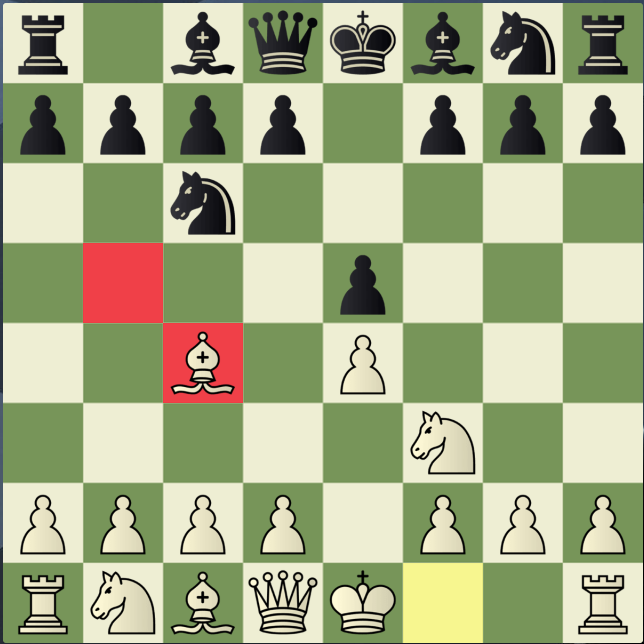
\includegraphics[width=\textwidth]{Images/Design/a-1.png}
            \caption{Italiana/Española} 
        \end{subfigure}
        \hfill
        \begin{subfigure}[b]{0.475\textwidth}  
            \centering 
            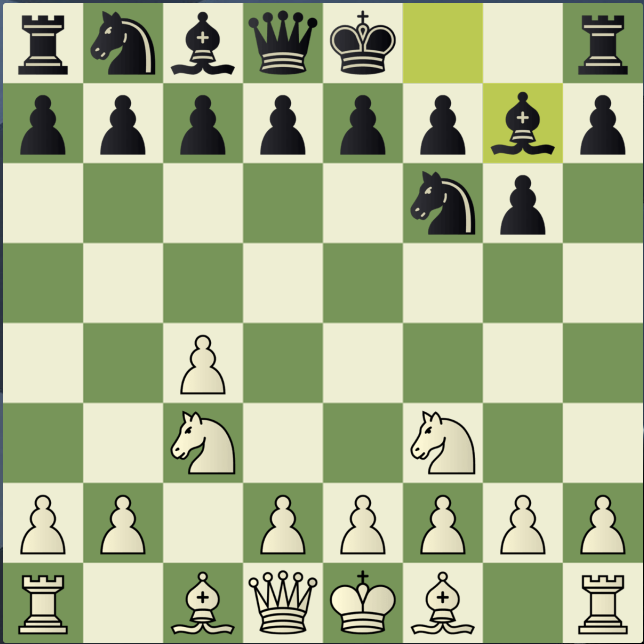
\includegraphics[width=\textwidth]{Images/Design/a-2.png}
            \caption{Inglesa}
        \end{subfigure}
        \vskip\baselineskip
        \begin{subfigure}[b]{0.475\textwidth}   
            \centering 
            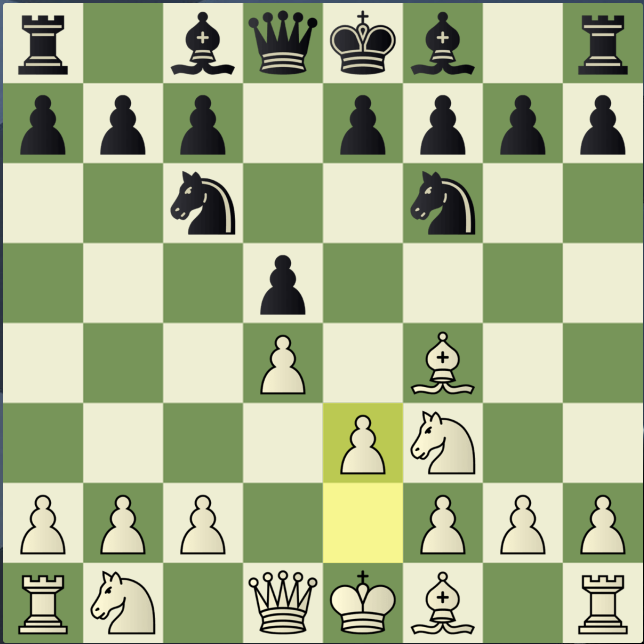
\includegraphics[width=\textwidth]{Images/Design/a-3.png}
            \caption{Sistema Londres}  
        \end{subfigure}
        \hfill
        \begin{subfigure}[b]{0.475\textwidth}   
            \centering 
            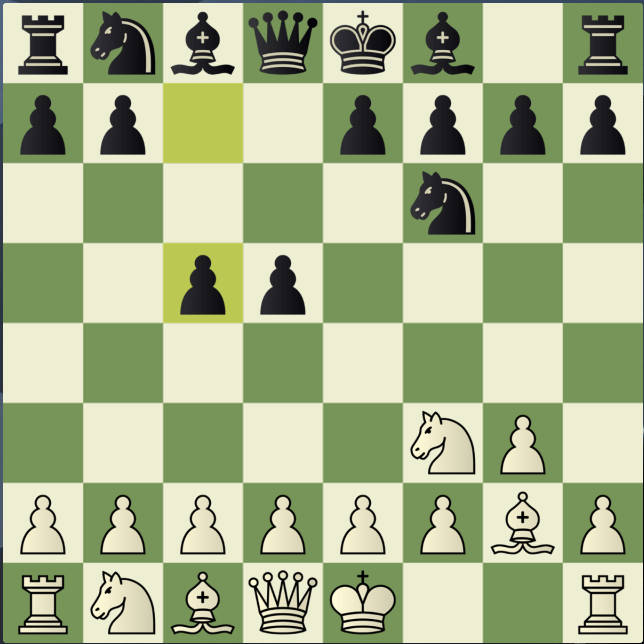
\includegraphics[width=\textwidth]{Images/Design/a-4.png}
            \caption{Fianchetto}  
        \end{subfigure}
        \caption{Aperturas comunes en ajedrez.}
    \end{figure*}
    \newpage 
\begin{figure*}[ht]
        \centering
        \begin{subfigure}[b]{0.475\textwidth}
            \centering
            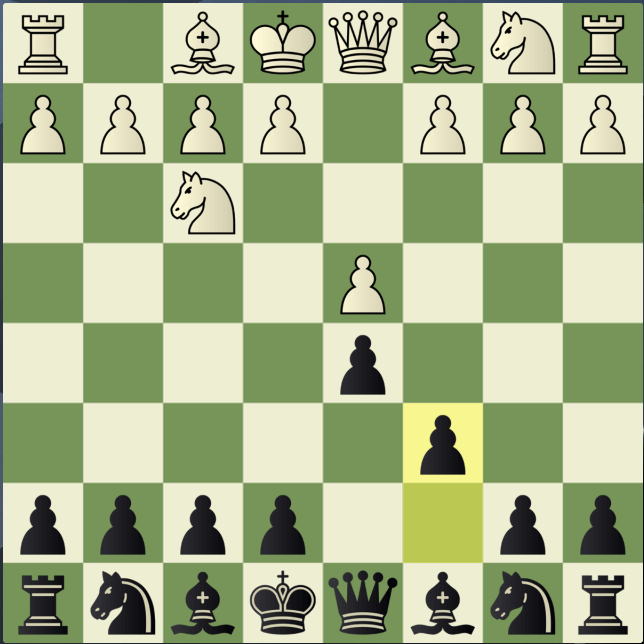
\includegraphics[width=\textwidth]{Images/Design/d-1.png}
            \caption{Eslava}
        \end{subfigure}
        \hfill
        \begin{subfigure}[b]{0.475\textwidth}  
            \centering 
            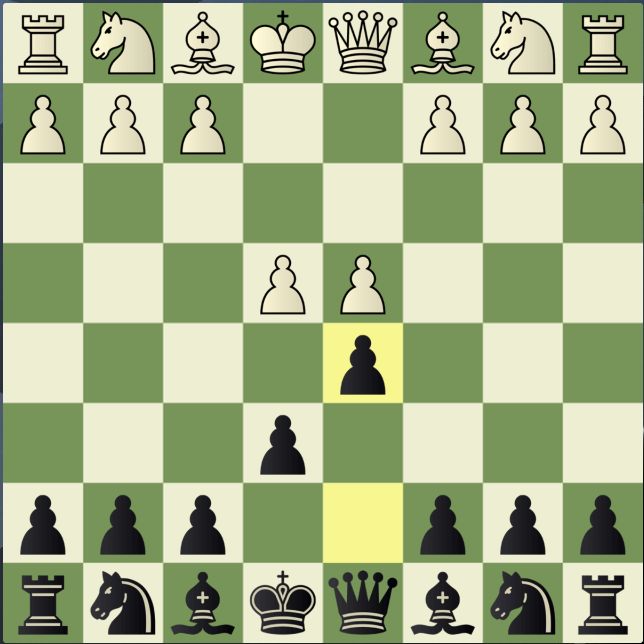
\includegraphics[width=\textwidth]{Images/Design/d-2.png}
            \caption{Francesa}
        \end{subfigure}
        \vskip\baselineskip
        \begin{subfigure}[b]{0.475\textwidth}   
            \centering 
            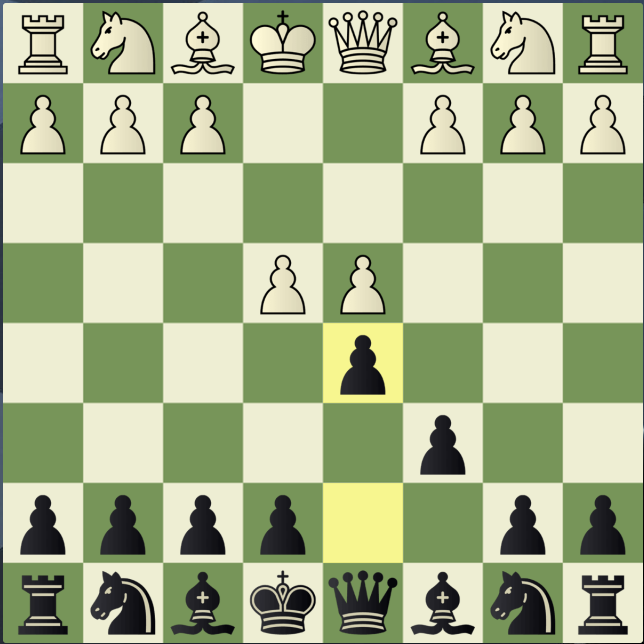
\includegraphics[width=\textwidth]{Images/Design/d-3.png}
            \caption{Caro-Kann}
        \end{subfigure}
        \hfill
        \begin{subfigure}[b]{0.475\textwidth}   
            \centering 
            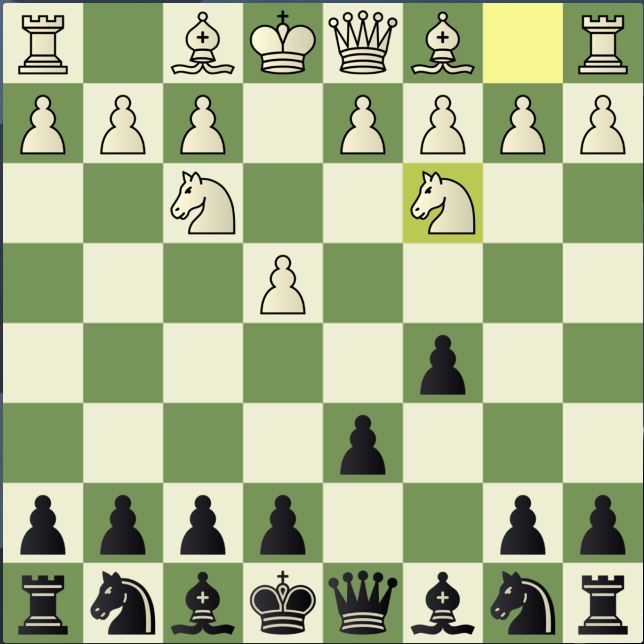
\includegraphics[width=\textwidth]{Images/Design/d-4.png}
            \caption{Siciliana}
        \end{subfigure}
        \caption{Defensas comunes en ajedrez.}
    \end{figure*}
    
    \newpage 